\section{Prepare your dissertation}
Here, we will explain what you need to do when writing a dissertation.

\subsection{Structure of dissertation}
The submitted dissertation must meet the following items.

\begin{enumerate}
    \item Title
    \item Author's name
    \item Affiliation (Program)
    \item Abstract
    \item Keywords (4-5 words)
    \item Thesis committee
    \item Text (including ``introduction'' and ``conclusion'')
    \item Acknowledgements (if necessary)
    \item Reference
    \item Publication list (if necessary)
    \item Appendix (if necessary)
    \item All figures, photographs, tables, and their captions
\end{enumerate}

\subsection{Abstract and Keyword}

Make an English abstract and English keywords. In addition, the title, author, thesis committee, and affiliation are shown.

\subsection{Page layout}
The page layout is shown in Fig. \ref{fig:layout}.
The top, bottom, left, and right margins are
0.5 cm, 0.5 cm, 0.6 cm, and 0.6 cm, respectively.
The height and width of the textbody are 20.5 cm and 14.5 cm, respectively.
The font size is 12 pt. The line spacing is 1.2×.

\begin{figure}[t]
    \centering
    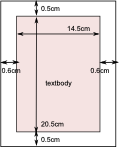
\includegraphics{src/Picture1.png}
    \caption{Page layout.}
    \label{fig:layout}
\end{figure}

\subsection{Figures, pictures, and tables}

\begin{enumerate}
    \item Use the figures, photographs, and tables originally created by the author. m in the figure in the text, indicate the corresponding English term in parentheses after the Japanese term if necessary.
    \item Insert figures, photographs, and tables together with their Japanese and English titles at appropriate positions in the text.
    \item If there are characters in the figure or photo, create them so that they can be identified by the size at the time of printing.
\end{enumerate}

The examples of figure and table are shown in Fig. \ref{fig:abyssinian} and Table \ref{tab:table}.

\begin{table}[t]
    \centering
    \caption{Table type styles}
    \begin{tabular}{c|c|c|c} \hline
        \multirow{2}{1cm}{Table Head} & \multicolumn{3}{|c}{Table column head} \\ \cline{2-4}
         & Table column subhead & Subhead & Subhead \\ \hline\hline
        copy & More table copy & & \\ \hline
    \end{tabular}
    \label{tab:table}
\end{table}

\begin{figure}[t]
    \centering
    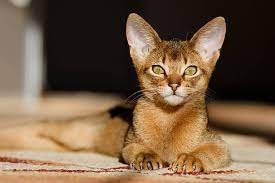
\includegraphics{src/abyssinian.jpeg}
    \caption{Abyssinian.}
    \label{fig:abyssinian}
\end{figure}

\subsection{Reference}
List and cite the references according to the style shown in
\cite{NIPS2012_c399862d}.